\documentclass[conference,final]{IEEEtran}

\usepackage{latex8}
\usepackage{times}

\usepackage[utf8]{inputenc}
\usepackage{graphicx}
\usepackage{url}
\usepackage{float}
\usepackage{times}    
\usepackage{multirow}    
\usepackage{listings}   
\usepackage{times}     
\usepackage{paralist}    
\usepackage{wrapfig}    
\usepackage[small,it]{caption}
\usepackage{multirow}
\usepackage{ifpdf}


\usepackage{listings}
\usepackage{keyval}  
\usepackage{color}
\definecolor{listinggray}{gray}{0.95}
\definecolor{darkgray}{gray}{0.7}
\definecolor{commentgreen}{rgb}{0, 0.4, 0}
\definecolor{darkblue}{rgb}{0, 0, 0.4}
\definecolor{middleblue}{rgb}{0, 0, 0.7}
\definecolor{darkred}{rgb}{0.4, 0, 0}
\definecolor{brown}{rgb}{0.5, 0.5, 0}

\lstdefinestyle{myListing}{
  frame=single,   
  backgroundcolor=\color{listinggray},  
  %float=t,
  language=C,       
  basicstyle=\ttfamily \footnotesize,
  breakautoindent=true,
  breaklines=true
  tabsize=2,
  captionpos=b,  
  aboveskip=0em,
  belowskip=-2em,
  %numbers=left, 
  %numberstyle=\tiny
}      

\lstdefinestyle{myPythonListing}{
  frame=single,   
  backgroundcolor=\color{listinggray},  
  %float=t,
  language=Python,       
  basicstyle=\ttfamily \footnotesize,
  breakautoindent=true,
  breaklines=true
  tabsize=2,
  captionpos=b,  
  %numbers=left, 
  %numberstyle=\tiny
}

\newcommand{\up}{\vspace*{-1em}}
\newcommand{\upp}{\vspace*{-0.5em}}
\newcommand{\numrep}{8 }
\newcommand{\samplenum}{4 }
\newcommand{\tmax}{$T_{max}$ }
\newcommand{\tc}{$T_{C}$ }
\newcommand{\bj}{BigJob}

\title{SAGA BigJob: An Extensible, Interoperable and General-Purpose
  Pilot-Job Abstraction for Distributed Applications and Systems}

\author{
Andr\'e Luckow$^{1}$, Lukasz Lacinski$^{1}$,   Shantenu Jha$^{1,2,3,*}$,\\
  \small{\emph{$^{1}$Center for Computation \& Technology, Louisiana State University, USA}}\\
  \small{\emph{$^{2}$Department of Computer Science, Louisiana State University, USA}}\\
  \small{\emph{$^{3}$e-Science Institute, Edinburgh, UK}}\\
  \small{\emph{$^{*}$Contact Author: \texttt{sjha@cct.lsu.edu}}}\\
}

%\date{}

\def\acknowledgementname{Acknowledgements}
\newenvironment{acknowledgement}%
{\section*{\acknowledgementname}%
\parindent=0pt%
}

\newif\ifdraft
\drafttrue
\ifdraft
\newcommand{\llnote}[1]{ {\textcolor{green} { ***JK: #1 }}}
\newcommand{\alnote}[1]{ {\textcolor{blue} { ***AL: #1 }}}
\newcommand{\jhanote}[1]{ {\textcolor{red} { ***SJ: #1 }}}
\else
\newcommand{\llnote}[1]{}
\newcommand{\alnote}[1]{}
\newcommand{\jhanote}[1]{}
\fi

\begin{document} 

\maketitle    

\begin{abstract}
  The uptake of distributed infrastructures by scientific applications
  has been limited by the availability of extensible, pervasive and
  simple to use abstractions which are required at multiple levels --
  development, deployment and execution stages of scientific
  applications. The Pilot-Job abstraction has been shown to be an
  effective abstraction to address many requirements of scientific
  applications.  Specifically, Pilot-Jobs support the decoupling of
  workload submission from resource assignment; this results in a
  flexible execution model, which in turn enables the distributed
  scale-out of applications on multiple and possibly heterogeneous
  resources.  Most Pilot-Job implementations however, are tied to a
  specific infrastructure. In this paper, we describe the design and
  implementation of a SAGA-based Pilot-Job, which supports a wide
  range of application types, and is usable over a broad range of
  infrastructures, i.e., it is general-purpose and pervasive, and as
  we will argue is also extensible to Clouds.  In this paper, we
  discuss how SAGA-based Pilot-Job is used for different application
  types and supports the concurrent usage across multiple
  heterogeneous distributed infrastructure, including concurrent usage
  across Clouds and traditional Grids/Clusters.  % Clouds provide a
%   different resource provisioning models from classical Grids.
  We discuss how Pilot-Jobs help support dynamical execution models
  and thus introduce new opportunities for distributed applications.
  We also demonstrate for the first time that we are aware of, the use
  of multiple Pilot-Job implementations to solve the same problem;
  specifically, we use SAGA to access the SAGA-based Pilot-Job on
  high-end resources such as the TeraGrid, whilst using the native
  Condor Pilot-Job (Glide-in) on Condor resources. Importantly both
  are invoked via the same interface without changes at the
  development or deployment level, but only an execution (run-time)
  decision.
% \alnote{I would propose to
  % describe which requirements of distributed apps are particularly
  % addressed by Pilot-Jobs}\jhanote{I have done so now in the 3rd and
  % 4th sentence. OK?}
\end{abstract}

% \up \up

% \section*{Structure/Outline}

% Section 1. Introduction -- talk about (i) Distributed Systems, need
% for abstractions (development, deployment and execution) and
% programming systems. (ii) Talk about Pilot-Jobs as one of the most
% successful ``execution abstraction''. (iii) Talk about limitations
% of current approaches. (iv) In a nutshell what this paper aims to
% achieve and then conclude with an outline.

% \bigskip

% Section 2. SAGA-based Pilot Job.  SAGA in brief. Place canonical SAGA
% picture. Talk about why using SAGA for PilotJob is different
% (integrated and consistent API). Talk about SAGA Job-Model; talk about
% extensions to the SAGA Job Model for BigJob.  Architecture and Control
% Flow for BigJob. Discuss how SAGA BigJob works well with Condor
% Glide-in.

% \bigskip 

% Section 3. Introduce Clouds -- SAGA for Clouds and parallel jobs for
% Clouds. Explain the role of a Pilot Job for Clouds. What does it mean?
% How is it different from Pilot Jobs for Grids/Clusters?  Talk about
% Parallel jobs and Clouds and how we manage them.

% \bigskip 

% Section 4. Usage Modes and Analysis: Already laid out.

% \bigskip 

% Section 5. Conclusion

% \jhanote{We need to be consistent with the usage of sub-job and
%   Sub-Job and subjob/SubJob. Preference?}

% \alnote{What spelling convention should we use: Pilot-Job, Big-Job, Sub-Job or PilotJob, BigJob, SubJob?}

\section{Introduction}

Infrastructure capabilities (tools, programming systems) and policy
determine applications, type development \& execution

1 Range of tools, prog. systems and environments large further adding
to challenges of providing Interoperability and extensibility 

2 Commonly accepted abstractions not available, Pilot-Job powerful,
but no “unifying” tool on TG

3 Deployment and execution challenges disjoint from the development
process: 

4 Dist. Application and Programming Systems and Tools 
 - Incompleteness and/or out-of-phase:  Need X and Y, but only X or Y available, 
   e.g., Master-Worker paradigm supported, but no FT.
 - Customization
 - Robustness and Scalability: Works well in small or controlled
 environment, but not at-Scale

 Will not be possible always, but extensibility and interoperability
 must be built into it as a fundamental design objective

DGI and PS/T need to account for the following characteristics of DA
 - Performance Models more than just simple HPC or peak-usage
 - Very broad range of usage modes that often need to be supported

Ironically, most applications have been developed to hide from
heterogeneity and dynamism; not embrace them Good heterogeneity vs
bad heterogeneity Dynamism: Performance Advantages The SAGA based
Pilot-Job provides supports for the good heterogeneity while
addressing the bad heterogeneity

Many applications have used distributed infrastructure to advance
understanding in their disciplines. A number of applications have been
able to use existing programming systems and tools, without having to
worry about customized extensions. However, there also exist a number
of applications that have had to implement new capabilities at one or
more levels, i.e., at the application, programming system, middleware,
and/or infrastructure level.  

... developers prefer to ``roll out their own" capabilities, even
though there exist programming systems with similar capabilities..

Different facets of extensibility: (i) new functionality, (ii) new
application domains and usage-modes (``put it out there and it will be
used in unexpected ways'') (iii) new infrastructure, (iv) scale-out?
(v) developer versus external user...

% Utilizing existing programming systems would enable the developer to
% focus on specifics of the application, rather than the implementation
% of such core infrastructure.

The lack of reusability and extensibility thus has the effect of
further suppressing distributed application development. Thus, it can
be asked in this context, why have application developers not
considered using capabilities from an existing programming system to
support the required capability? This may be due to a number of
factors: (a) Many programming systems lack robustness when used by
developers in scientific applications -- for instance, they may have
limits on scalability. (b) The level of maturity and development
schedule of the programming system may not align with the requirements
of the application developers. (c) It may be difficult to isolate a
specific capability from a programming system, thereby limiting re-use
by an application developer requiring that capability. In
general~\cite{dpagrid2009} programming systems fall short of the
requirements of distributed applications due to: {\em
  i. Incompleteness:} Programming systems and tools are often
incomplete or inflexible with respect to application needs, e.g.,
tools that support the master-worker paradigm often only address
failures of workers and not of the master. Furthermore, they may not
address non-functional issues such as security and privacy, which may
be critical for some applications.  {\em ii. Customization:}
Programming systems and tools also tend to be customized to
applications and their requirements, with limited concern for reuse or
extensibility.  Applications and tools are also often highly dependent
on (and tuned to) a specific execution environment, further impacting
portability, re-usability, and extensibility.

The level of success of these efforts depended not only on the
resulting programming system, but also on the suitability of the
underlying paradigm for Grid environments. The Pilot-Job abstraction
has been widely used and interestingly used across several different
PGI. However, they are all customized Pilot-Job implementations, often
tightly coupled/tied to a specific infrastructure, and not extensible
or usable across different systems...

\emph{Pilot-Jobs} is an execution abstraction that has been used by
many communities to increase the predictability and time-to-solution
of such applications. A Pilot-Job allows the execution of jobs without
the necessity to queue each individual sub-job. The Pilot-Job itself
is a regular Grid job, which is started through a Grid resource
manager, such as the Globus GRAM.  Pilot-Jobs are, (i) used to improve
the utilization of resources, (ii) to reduce the net wait time of a
collection of tasks (iii) facilitate bulk or high-throughput
simulations where multiple jobs need to be submitted which would
otherwise saturate the queuing system, (iv) as a basis to implement
application specific scheduling decisions and policy decisions.
Discuss PilotJob: (i) How Traditionally Used (mostly deployment time);
(ii) Advantages; (iii) How traditionally bound to a single platform
and system.

For example, on the LHCb computing model, Grid jobs are routed through
the DIRAC~\cite{dirac} workload management system (WMS). DIRAC is a
pilot-based system where user jobs are queued in the WMS server and
the server submits generic pilot scripts to the Grid. Each pilot
queries the WMS for a job with resource requirements satisfied by the
machine where the pilot script is running. If a compatible job is
available, it is pulled from the WMS and started. Otherwise, the pilot
terminates and the WMS sends a new pilot to the Grid. This system
improves the reliability of the Grid system as seen by the user.  the
DIRAC system was developed in order to provide a complete solution for
using the distributed computing resources of the LHCb experiment at
CERN for data production and analysis. It allows a concurrent use of
over 10K CPUs and 10M file replicas distributed over many tens of
sites.  There can be additional functionality that builds upon a
pilot-based scheme; for example DIANE~\cite{diane} a lightweight
agent-based scheduling layer can use DIRAC.

The Simple API for Grid Applications (SAGA) is a high-level,
easy-to-use API for accessing distributed resources. Unlike other
common Pilot-Job systems SAGA BigJob (i) natively supports MPI job and
(ii) works on a variety of back-end systems, generally reflecting the
advantage of using a SAGA-based approach.

Recently, the usage of virtualization and the usage of on-demand
virtual machines become increasingly popular. These so-called
infrastructure-as-a-service Clouds have different advantages compared
to traditional Grid systems: users are provided with a greater
flexibility and have the ability to customize their virtual machine
environment. At the same time virtual machines are well isolated from
each other. More and more the need to integrate traditional Grids and
Clouds arises.

Developing and running applications in such a hybrid and dynamic
computational infrastructure presents new and significant
challenges~\cite{cloud-grid-autonomics}. These include the need for
programming systems that can express the hybrid usage modes and
associated runtime trade-offs and adaptations, as well as coordination
and management infrastructures that can implement them in an efficient
and scalable manner. Key issues include decomposing applications,
components and workflows, determining and provisioning the appropriate
mix of Grid/Cloud resources, and dynamically scheduling them across
the hybrid execution environment while satisfying/balancing multiple,
possibly changing objectives for performance, resilience, budgets and
so on.

\section{Related Work} %\jhanote{AL, SJ}

As more applications try to adopt the advantages from dynamic
execution, the Pilot-Job concept has grown in popularity and has been
extensively researched and implemented for different usage scenarios
and infrastructure. % Different systems that use similar Glide-In
% approaches have been developed. 
% Frey et al.~\cite{citeulike:291860} initially proposed this idea in
% their work on Condor Glide-In. 
Using Condor Glide-In a complete Condor pool can be initiated using
the GRAM service.  Falkon~\cite{1362680} is a newer system, which
emphasize in particular the performance of its task
dispatcher. However, both systems have limitations and impose
different overheads: Condor Glide-In~\cite{citeulike:291860} requires
the start of a complete set of Condor daemons within the allocated set
of resources. Falkon does not support MPI applications, i. e. it is
not usable for our application scenario.

Nimbus~\cite{10.1109/MIC.2009.94} provides a Pilot-Job like
abstractions for Clouds. For this purpose, Nimbus allows the launch of
auto-configured virtual machine clusters that contain a Torque and
Globus installation.  The Atlas computing framework developed at CERN
also heavily relies on the PanDA Pilot-Job framework to implement
resource leases. Using the VIRM API, PanDA was extended to support
different virtualization backends, e.\,g.\ OpenNebula and
Nimbus. However, in contrast to the SAGA-based Pilot
Job for Clouds, both frameworks are strongly coupled to a particular
backend infrastructure -- Globus in the case of Nimbus and gLite in
the case of PanDA. The advantage of the SAGA Pilot-Job is that it
allows applications to seamlessly utilize different backend
infrastructure, e.\,g.\ Condor, Globus and different kinds of Clouds,
at the same time.


% Further, Nimbus provides a possibility to integrate classical batch clusters
% and VM clusters. By running cluster in a hybrid mode this setup 
% can support both native jobs by running those in the Xen's
% domain 0 as well as VMs. However, only in the VM usage mode, the user is
% able to control the entire setup and configuration of its virtual machines.


\section{SAGA and SAGA-based Frameworks for Large-Scale and
  Distributed Computation} \jhanote{AL, SJ}

\alnote{removed the first paragraph - duplicated content}
% SAGA~\cite{saga_url} provides a simple, POSIX-inspired API to the most
% commonly required distributed functionality at a sufficiently
% high-level of abstraction so as to be independent of the divers\ e and
% dynamic Grid environments.

The Simple API for Grid Applications (SAGA)~\cite{saga_url} is an API
standardization effort within the Open Grid Forum
(OGF)~\cite{saga_gfd90}, an international standards development body
concerned primarily with standards for distributed computing. SAGA
provides a simple, POSIX-style API to the most common Grid functions
at a sufficiently high-level of abstraction so as to be independent of
the diverse and dynamic Grid environments. The SAGA specification
defines interfaces for the most common Grid-programming functions
grouped as a set of functional packages (Fig.~\ref{Fig:SAGA1}). Some
key packages are:

\begin{figure}[!ht]
 \begin{center}
     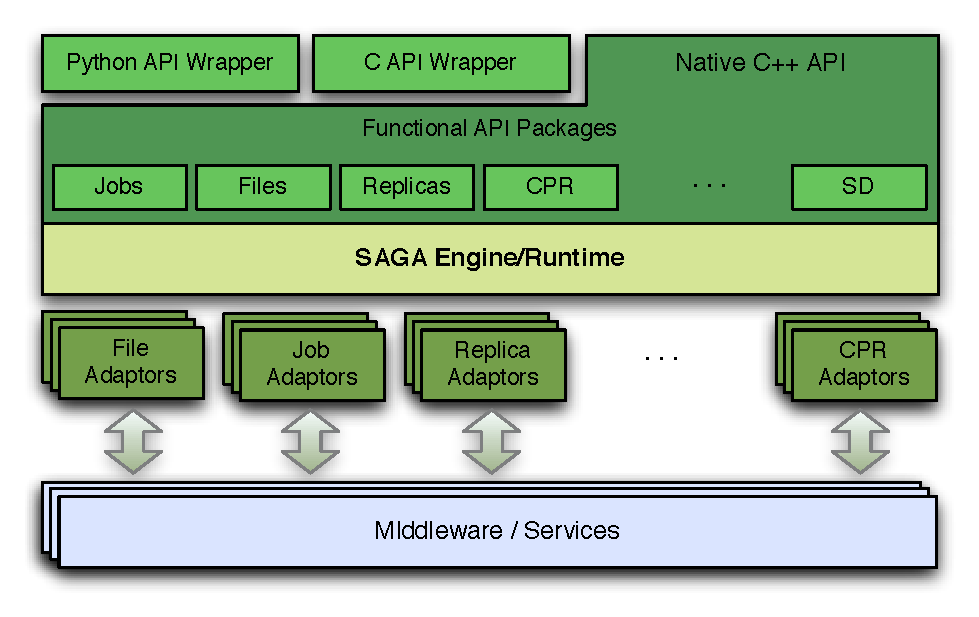
\includegraphics[width=0.40\textwidth]{stci_saga_figures-1.pdf}
 \end{center}
\caption{\small Layered schematic of the different components of the
   SAGA landscape. At the topmost level is the simple integrated API
   which provides the basic functionality for distributed
   computing. Our BigJob abstraction is built upon this SAGA layer
   using Python API wrapper} \label{Fig:SAGA1}
\end{figure}

\begin{itemize}
\item File package - provides methods for accessing local and remote
 filesystems, browsing directories, moving, copying, and deleting
 files, setting access permissions, as well as zero-copy reading and
 writing
\item Job package - provides methods for describing, submitting,
 monitoring, and controlling local and remote jobs. Many parts of
 this package were derived from the largely adopted
 DRMAA % ~\cite{drmaa_url}                                                                                           
 specification.
\item Stream package - provides methods for authenticated local and
 remote socket connections with hooks to support authorization and
 encryption schemes.
\item Other Packages, such as the RPC (remote procedure call) and Replica
 package
\end{itemize}

In the absence of a formal theoretical taxonomy of distributed
applications, Fig.~\ref{Fig:sagaapps} can act a guide.  Using this
classification system, there are three types of distributed
applications: (i) Applications where local functionality is swapped
for distributed functionality, or where distributed execution modes
are provided.  A simple but illustrative example is an ensemble of an
application that uses distributed resources for bulk submission. Here,
the application remains unchanged and even unaware of its distributed
execution, and the staging, coordination, and management are done by
external tools or agents. Most application in this category are
classified as implicitly distributed.  (ii) Applications that are
naturally decomposable or have multiple components are then aggregated
or coordinated by some unifying or explicit mechanism.  DAG-based
workflows are probably the most common example of applications in this
category.
    % (ii) Applications that are developed using well known patterns,                                                
    % for example MapReduce, which in turn is implemented using                                                      
    % infrastructure independent programming systems such as SAGA;                                                   
Finally, (iii) applications that are developed using frameworks, where
a framework is a generic name for a development tool that supports
specific application characteristics (e.g., hierarchical job
submission), and recurring patterns (e.g., MapReduce, data
parallelism) and system functionality.  SAGA has been used to develop
system-level tools and applications of each of these types.

\begin{figure}[!ht]
  \begin{center}
    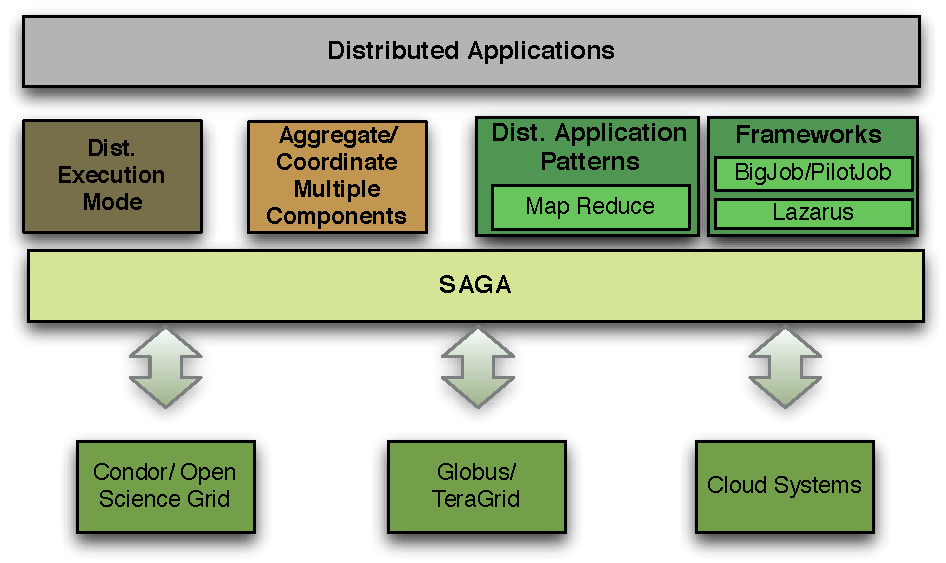
\includegraphics[width=0.45\textwidth]{distributed_applications_saga_figure.pdf}
  \end{center}
  \caption{\small Showing the ways in which SAGA can be used to
    develop distributed applications.  The different shaded box
    represent the three different types; frameworks in turn can
    capture either common patterns or common application
    requirements/characteristics. \label{Fig:sagaapps} }
\end{figure}

It is important to note that SAGA provides the basic API to
implement distributed functionality required by applications
(typically used directly by the first category of applications),
and is also used to implement higher-level APIs, abstractions, and
frameworks that, in turn, support the development, deployment and
execution of distributed
applications~\cite{enkf-gmac09,saga_data_intensive_abstractions}. In
Ref.~\cite{sagamontage09} we discussed how SAGA was used to
implement a higher-level API to support workflows. In this paper, 
we will discuss how SAGA can be used to implement runtime
frameworks to support the efficient execution of the distributed
applications.


\section{BigJob -- The SAGA-based Pilot-Job} \jhanote{AL}
Pilot-Jobs are a useful abstraction for efficiently executing an
ensemble of batch jobs without the necessity to queue each individual
job. A Pilot-Job is a normal Grid job, which is places into the batch
queue of the respective Grid resource. Once the batch queue assigned
the requested resources to the Pilot-Job, the Pilot-Job is responsible
for managing these and assigning them to so-called sub-jobs.  That way
queuing times for sub-jobs can be reduced and the predictability for
application scenarios can be increased.


Pilot-Jobs decouple resource allocation from resource binding and
allow the efficient utilization of resources. By delaying the resource
binding decision into the application-level, dynamic usage modes,
e.\,g.\ the load-depended sizing of sub-jobs or the dynamic addition
of resources to meet deadlines, can be supported.

\emph{BigJob} is a SAGA-based Pilot-Job implementation. In contrast to other
Pilot-Job implementations as Condor Glide-In or Falkon, BigJob
natively supports parallel applications (e.g. based on MPI) and works
independent of the underlying Grid infrastructure across different
heterogeneous backend, e.\,g.\ Grids and Cloud, reflecting the
advantage of using a SAGA-based approach. 

As shown in Figure~\ref{fig:figures_distributed_pilot_job} BigJob provides
a unified abstraction to Grids, Condor pools and Clouds. Using the same API,
applications can dynamically allocate resources via the big-job interface and
bind sub-jobs to these resources. In the next sections the three different backends
will be described.
\begin{figure}[htbp]
    \centering
        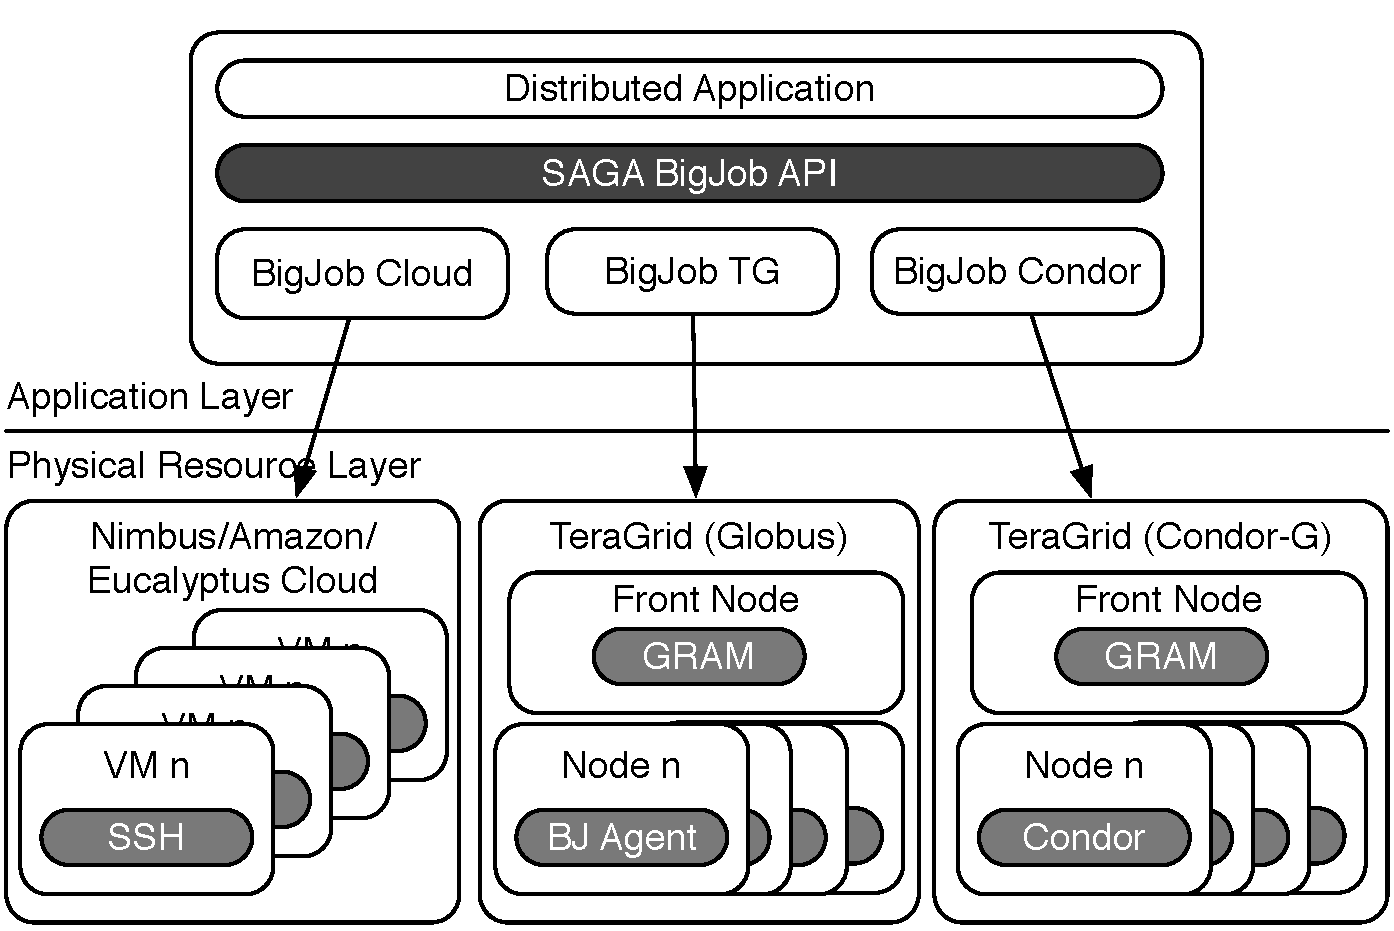
\includegraphics[width=0.45\textwidth]{figures/distributed_pilot_job}
    \caption{\textbf{Overview of the SAGA-based Pilot Job:} The SAGA Pilot Job API is
    currently implemented by three different backends - one for Grids, Condor and 
    for Clouds.}
    \label{fig:figures_distributed_pilot_job}
\end{figure}

\alnote{Old Notes: 
Introduce BigJob:
 - Describe it, and how it differs from other PilotJobs
 - Outline new usage modes that BigJob fundamentally supports:
    -- As the basis for scale-out across
    -- As the basis for a framework for runtime optimization
    -- More thought?
BigJob:
 - Architecture and control flow details
 - Performance Numbers}

\subsection{BigJob for Grids}

Figure~\ref{fig:figures_bigjob} shows an overview of the SAGA BigJob 
implementation for computational Grids. The Grid BigJob comprises 
of three components: (i) the BigJob Manager that
provides the Pilot-Job abstraction and manages the orchestration and
scheduling of BigJobs (which in turn allows the management of both
BigJob objects and subjobs) (ii) the BigJob Agent that represents the
pilot job and thus, the application-level resource manager on the
respective resource, and (iii) the advert service that is used for
communication between the BigJob Manager and Agent.

\begin{figure}[ht]
    \centering
    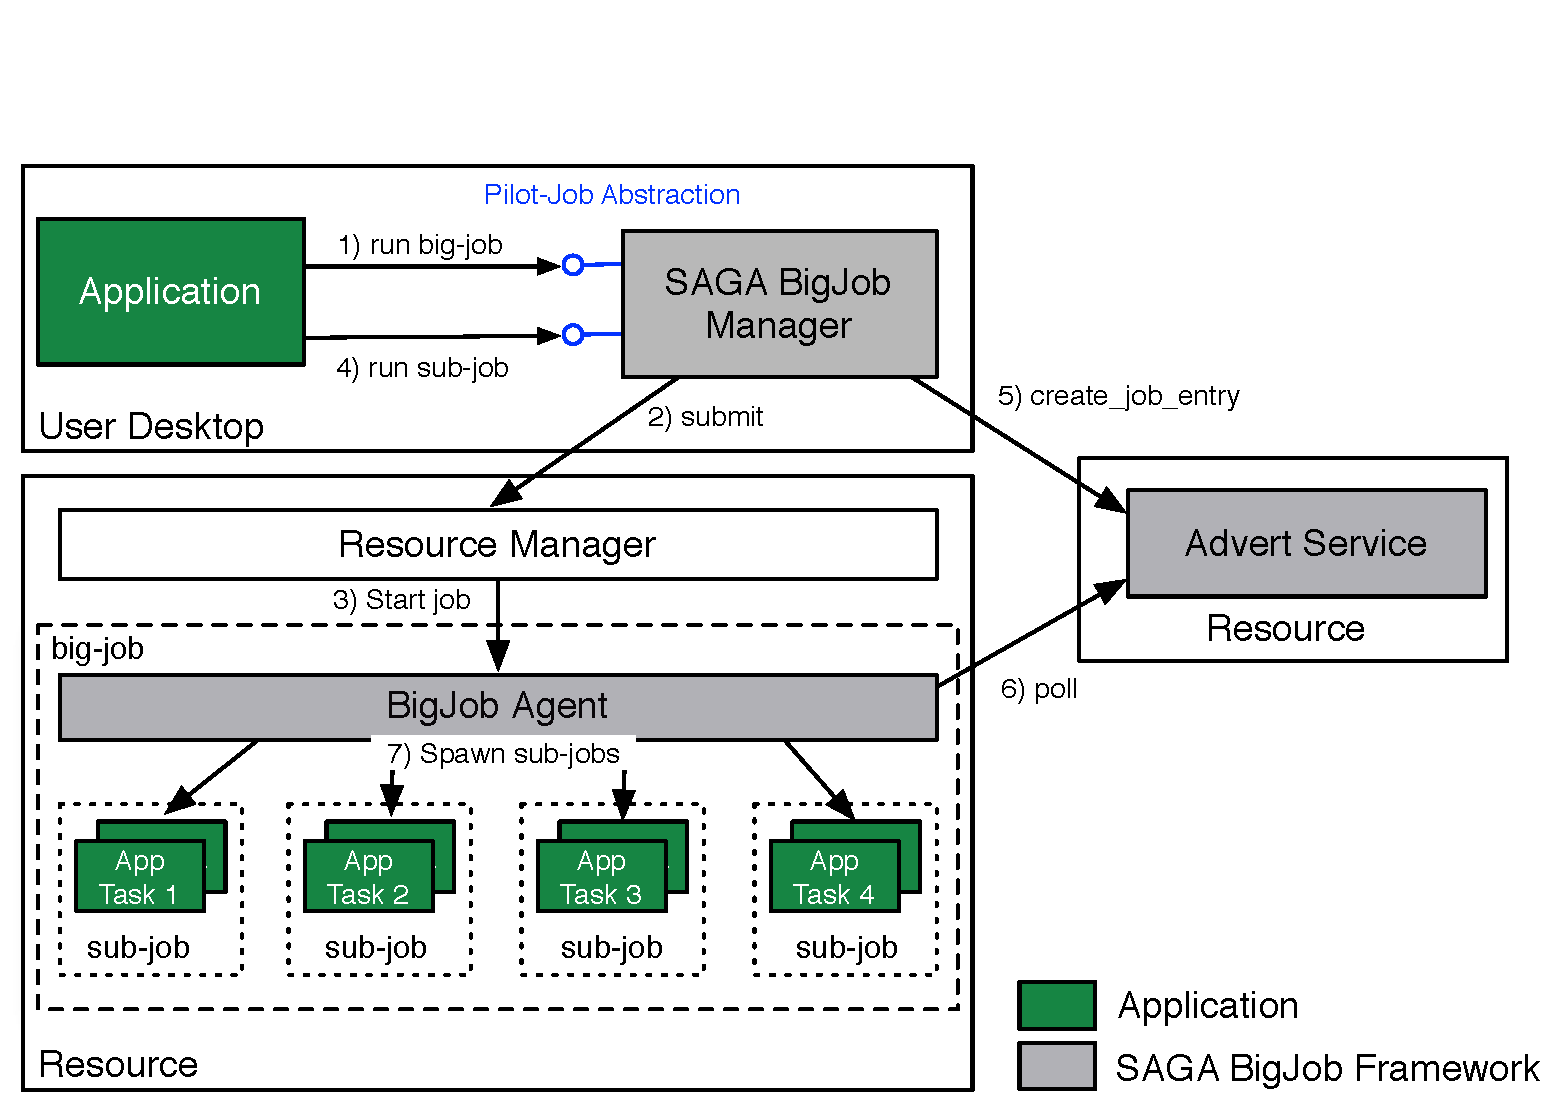
\includegraphics[width=0.45\textwidth]{figures/bigjob}
   \caption{BigJob Architecture: The core of the framework, the
      BigJob Manager, orchestrates a set of sub-jobs via a
      BigJob Agent using the SAGA job and file APIs.  The
      BigJob Agent is responsible for managing and monitoring sub-jobs
      on a single machine.}
   \label{fig:figures_bigjob}
\end{figure}

Applications can utilize the framework via the big-job and
sub-job classes.  Before running regular jobs, an application
must initialize a big-job object.  The BigJob Manager then
queues a Pilot-Job, which actually runs a BigJob Agent on the
respective resource. For this agent a specified number of resources is
requested. Subsequently, sub-jobs can be submitted through the BigJob
Manager using the job-id of the BigJob as reference. The BigJob
Manager ensures that the subjobs are launched onto the correct
resource based upon the specified job-id using the right number of
processes. Communication between the BigJob Agent and BigJob Manager
is carried out using the SAGA advert service, a central key/value
store. For each new job, an advert entry is created by the BigJob
Manager. The agent periodically polls for new jobs. If a new job is
found and resources are available, the job is dispatched, otherwise it
is queued.

Need to mention that BigJob is based upon extensions to the SAGA job
and file APIs, and thus is both syntactically and semantically
consistent with the core SAGA package. Hence, referred to as a
SAGA-based framework.


\subsection{BigJob and Condor Glide-in} \jhanote{Lukas}


\jhanote{How bigjob works with Condor Glide-in}

Condor natively provides Pilot-Job functionality; in fact, Condor has
been instrumental in the uptake and popularization of the Pilot-Job
concept.
% that allows implement the general BigJob 
% architecture in many different ways. 
In fact the challenge here is to implement BigJob as an overlay over
Condor's native pilot-job with minimal disruption. The idea of Advert
Service as a central point of collecting information about sub-jobs
can be substituted by a Condor queue. This approach gives some
advantages.  BigJob can utilize Condor scheduling and matchmaking. It
allows the control in an unified way of the state of Pilot-Jobs and
sub-jobs as Condor jobs. The advert service still can be applied and
is an answer to a problem of central coordination point if many
different backends (Condor pool, Clouds, Grids) are used.  However the
approach presented here shows how to implement the BigJob idea
referring Condor only.

\begin{figure}[!ht]
 \begin{center}
     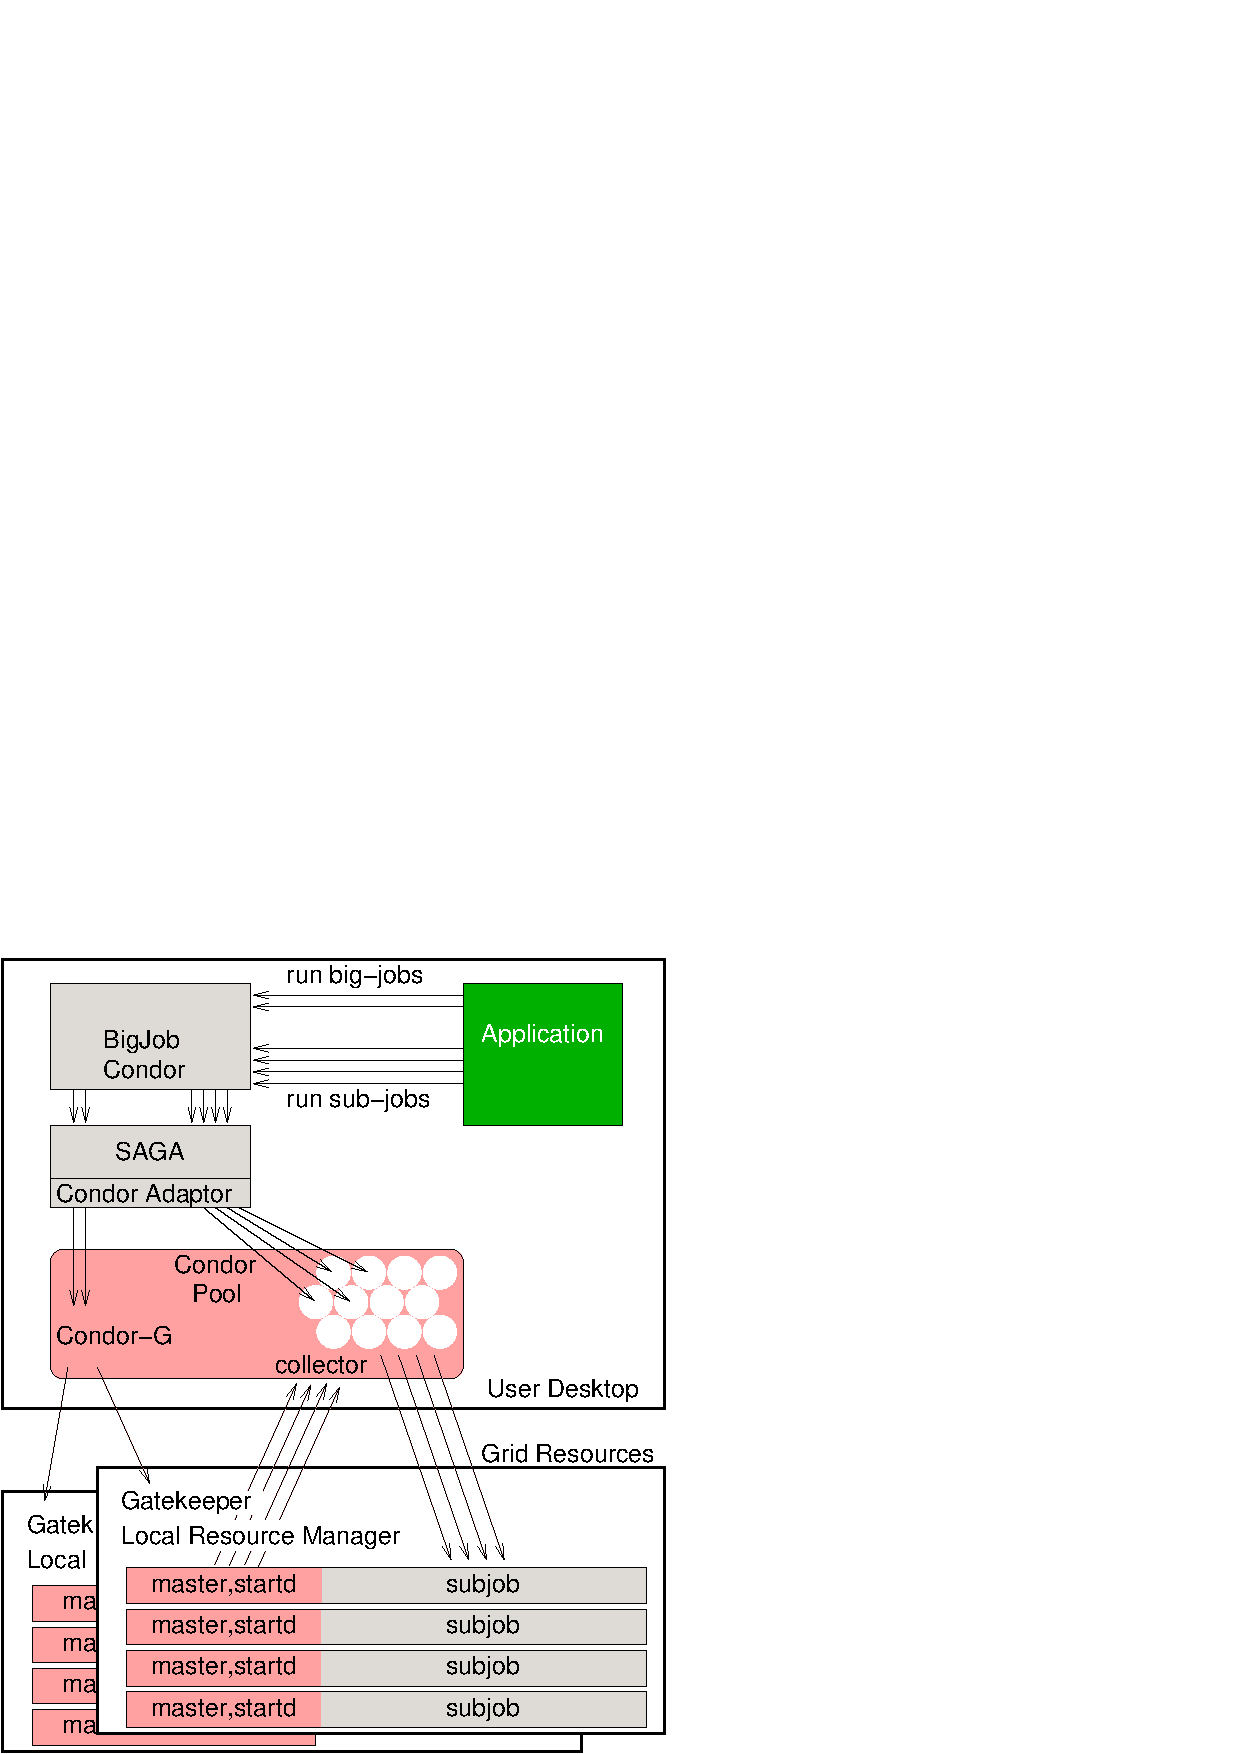
\includegraphics[width=0.33\textwidth]{figures/bigjob_condor}
 \end{center}
 \caption{\small Schematic showing how the BigJob interface is used to
   submit jobs to a Condor Glide-in without any changes in semantics
   or usage mode of the Condor Glide-in. The application submits the
   sub-jobs (which are the 8 replicas) to a BigJob object, which then
   submits to the available condor pool. The Condor Glide-in then
   takes responsibility of managing the resources that constitute the
   pool and distributing sub-jobs to them.} \label{fig:saga-condor}
\end{figure}

\jhanote{... such simple extensibility ... illustrates how SAGA
  enables the integration of heterogeneous resources to facilitate
  distributed Scale-out.??}

Figure~\ref{fig:saga-condor} illustrates the architecture of the Condor BigJob.
A Condor Pilot-Job from an application point of view is a request 
for a set of resources that can later be accessed via the local Condor pool. 
To initiate a Pilot-Job, the application must specify a GRAM endpoint 
of a Grid resource, a number of requested nodes and a wall time (step 1). 
The Condor Bigjob translates this request to a Condor-G job, which is managed
using the SAGA Condor adaptor. Condor is then responsible for submitting 
the job to the GRAM of the specified remote resource (step 3). Once the Condor-G
job becomes active, it start the Condor daemons \texttt{master} and \texttt{startd} on 
the remote resources (step 4). During the initialization these 
daemons register the allocated resources with the Condor
pool on the user's desktop creating a coherent computing resource to
submit sub-jobs to (step 5). As with the Grid BigJob sub-job objects
can be created via the Pilot-Job abstraction. The Condor BigJob maps these
sub-jobs to the Condor pool and starts them via the SAGA Condor adaptor (steps 6-8). 
Also, sub-jobs can already be submitted before any node joins the
Condor pool. These jobs will automatically wait until scheduler is able to find any
``Unclaimed'' resources matching a sub-job's requirements. 

Thanks to the native capabilities of the Condor Pilot-Job, the Condor BigJob
is able to support some enhanced features, e.\,g.\ the management
of multiple Pilot-Jobs per big-job object. This capability is in particular
useful since the usage of multiple clusters can reduce \tc for many application
scenarios. For example, if one of the requested clusters is heavily loaded, the
waiting time of the Pilot-Job can be very long. In general, the more resources used, the 
lower the time until the first Pilot-Job and thus, the first sub-jobs becomes
active 

% will be executed as soon as a first
% pilot-job starts and nodes of the least loaded cluster join the Condor
% pool.

\jhanote{Lukas, I have taken a quick pass at the above paragraph, but
  more is required. It is a bit difficult to read and understand, how
  BigJob works with Condor-Glide-in. Maybe in addition to the above
  control flow (which is helpful), add a few sentences about the
  mapping between BigJob's interface (API calls) and Condors? That
  might help.. Andre/Lukas: What do you think? ANy other suggestions
  for improving this section?}

\jhanote{We should make sample code, examples and data-sets available
  on our website. Simple packaging}

\subsection{BigJob for Clouds} \jhanote{AL}

% espite a standardized interface, big difference on how to obtain meta-data (internal ip etc.)

At the execution level, Clouds differ from Clusters/Grids in at least
a couple of different ways. In Cloud environments, user-level jobs are
not typically exposed to a scheduling system; a user-level job
consists of requesting the instantiation of a virtual machine (VM).
Virtual machines are either assigned to the user or not (this is an
important attribute that provides the illusion of infinite resources).
The assignment of job to a VM must be done by the user (or a
middleware layer as BigJob).  In contrast, user-level jobs on Grids
and clusters are exposed to a scheduling system and are assigned to
execute at a later stage.  Also a description of a Grid job
typically contains an explicit description of the workload; in contrast
for Clouds a user level job usually contains the container
(description of the resource requested), but does not necessarily
include the workload. In other words, the physical resources are not
provisioned to the workload but are provisioned to the container.
This model is quite similar to resource reservations where you obtain
a ``container'' of resources to which you can later bind jobs
to. Interestingly, at this level of formulation, Pilot-Jobs attempt to
provide a similar model of resource provisioning as Clouds natively
offer. The Cloud usage model naturally maps to the Pilot-Job abstraction 
where resource allocation is done within the big-job and the resource 
binding is conducted dynamically for each sub-job.

As shown in Figure~\ref{fig:figures_distributed_pilot_job} the Cloud BigJob implements
the Pilot-Job abstraction for Cloud resources. In the following, we discuss
the internals of the BigJob Cloud implementation. Initially it is required that the user
prepares and uploads a virtual machine image for respective Cloud environment. 
This image should contain the application and possibly the
application data. Once the image is setup, the user can initialize a
\texttt{bigjob\_cloud} object specifying the Cloud environment, 
the image-id of the prepared VM image as well as the number and type of the VMs. The 
BigJob Manager then starts up the VM cluster on the requested Cloud. 
For this purpose, the manager relies on a resource adaptor
for each Cloud. This adaptor encapsulates Cloud specifics, such as the used
security mechanism, the communication protocol and the required setup tasks. Currently,
Amazon EC2, Eucalyptus and Nimbus Clouds are supported. Despite some similarities
between these Clouds and the trend toward standardization on the
EC2 API, there are subtle differences, e.\,g.\ in the allocation
of IP addresses, the SSH key handling, the metadata management or 
the network setup. The Cloud BigJob attempts to hide these differences 
from the user. However, a further standardization of such Cloud environments, 
e.\,g.\ within the OCCI efforts~\cite{occi}, is necessary.

The Cloud BigJob supports basic fault tolerance features: failed requests e.\,g.\
are automatically re-executed $n$ times. If not sufficient resources can be
allocated, the BigJob changes to the state \emph{failed} and terminates all previously
started VMs. Once all requested resource have been successfully allocated, the BigJob manager
prepares each virtual machine for further job executions e.\,g.\ by setting
up all SSH keys, which is a pre-requisite for running MPI applications.
Having finished all preparation tasks, the BigJob changes into the state
\emph{Running}. 

After the running state has been reached, the manager starts to process sub-jobs.
Unprocessed sub-jobs are stored in a FIFO queue. As resources become available,
sub-jobs are assigned to these. For parallel jobs the manager generates
a nodefile, which is then used for launching the application. Once the preparation
work has been finished, the manager spawns the sub-job using the SAGA job API and the SSH
adaptor. The progress of all sub-jobs is monitored by the manager using the standard mechanisms 
provided by the SAGA job API and a monitoring thread. Once a job terminates, i.\,e.\ it changes 
to the state \emph{Done} or \emph{Failed}, the allocated resources are freed. 
A new sub-job from the queue can then be assigned to newly available resources.

Since all meta-data of the assigned Cloud virtual machines, in particular the internal
and external IPs of the VMs, is available via the Cloud APIs of the supported Cloud 
environments it is in contrast to the Grid BigJob not necessary to deploy any 
agents on the Cloud machines. The state of all VMs can simply be maintained by the 
manager; remote launching can be done via the SSH protocol.


\subsection{BigJob Overheads} \jhanote{All}

\alnote{Should we move this section to Usage Model and Analysis?}
\jhanote{I think not. The performance referred to here is that of just
  BigJob startup and dispatch time -- which in principle should be
  independent of any usage mode/scenario. Right?}

In the following the overheads resulting from the usage of BigJob within
Grid applications is analyzed. Typically, the main overhead 
when using BigJob results from the queueing time at
individual resources on a Grids respectively from the
virtual machine creation time in Cloud environments. 
Figure~\ref{fig:performance_setup_time} compares the startup time of the
different Pilot-Job backends for Grids, Condor pools and Clouds.
\begin{figure}[htbp]
    \centering
        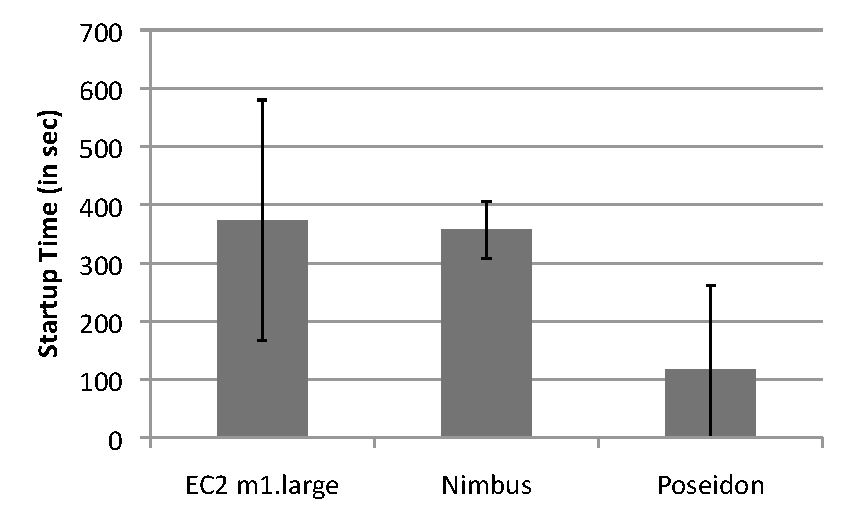
\includegraphics[width=0.45\textwidth]{performance/setup_time_xls.pdf}
    \caption{\textbf{BigJob Startup Times:} In Grids the startup time
      greatly depends upon the queuing time at the local resource
      manager. However, in our experiments also Clouds showed a high
      fluctuation in the queueing time.}
    \label{fig:performance_setup_time}
\end{figure}

Interestingly, the startup times for the Cloud environments have been larger than 
for the LONI resource Poseidon, which was very light loaded at the time
of the experiment. Obviously, the startup of a VM involves higher overheads 
than spawning a job on an already running machine: a resource for the VM 
must be allocated, the VM must be staged to the target and booted up. The following
experiments will also show that especially the already oversubscribed intra Cloud network
and thus, the staging of the VM can be a bottleneck. Also, there is a
large fluctuation in particular in the EC2 environment probably caused by 
the fact that insufficient resources have been available at certain times.

Also, Condor Glide-In and thus, the SAGA-Condor BigJob shows severe 
overheads compared to the Grid BigJob. These overheads can mainly be 
attributed to the Condor architecture. Condor requires to run several more or less 
lightweight daemons to be run on the target resource. The overhead is mainly 
cause by the time required to setup the pool, propagate the pool information 
to the main Condor pool and the Condor matchmaking, resource allocation and 
job spawning mechanism. A major advantage of the SAGA-based BigJob is that
it not only works across different infrastructures, it also provides a superior
performance and less overheads than Condor Glide-In.

In the following section we show that the SAGA BigJob abstraction is
suitable for running Pilot-Jobs on different kinds of distributed
infrastructures supporting different usage modes.

\section{Usage Modes and Analysis}


The aim of this section is not to perform detailed systematic
performance measures and analysis, but to illustrate the various usage
modes the SAGA-based BigJob can support and to explain how they are supported. We
posit that the performance overheads of BigJob are small relative to
the duration of the tasks that are typically performed, i.e., order of
seconds compared to tens of minutes and hours.  Needless to say, if
millions of jobs each of short duration were being attempted then the
overheads would be significant.

We discuss two scenarios that are representative of how applications
would typically use multiple distributed infrastructures. We focus our
attention on replica-based MD simulations and define a workload as
\numrep replicas of the HCV model~\cite{}, each replica running for
500 timesteps.  The first scenario involves running all \numrep over
different infrastructure configurations and determining the \tc for
each scenario. We repeat \tc for each configuration \samplenum times.

The second scenario, introduces an upper-bound on the acceptable \tc
(defined as \tmax) -- which is the maximum permissible time to
solution.

Each scenario has several possible specific sub-scenarios, of which we
discuss a few in each.

\subsection{Test Application: Hepatatis-C Virus (RNA) Using
  Replicas}

Several classes of applications are well suited for distributed
environments. Probably the best known and most powerful examples are
those that involve an ensemble of decoupled tasks, such as simple
parameter sweep applications~\cite{1239909}. Here we outline a
scientific basis for focussing on an ensemble of (parallel HPC)
Molecular Dynamics (MD) simulations.  Sufficient sampling of
configurations is an important requirement for MD simulations in order
to connect atomistic results to macroscopic or thermodynamic
quantities available from experiments.  Ensemble based approaches
represent an important and promising attempt to overcome the general
limitations of insufficient time-scales, as well as specific
limitations of inadequate conformational sampling arising from kinetic
trappings.  The fact that one single long-running simulation can be
substituted for an ensemble of simulations, make these ideal
candidates for distributed environments.  This thus provides an
important general motivation for researching ways to support scale-out
and thus enhance sampling and to thereby increase ``effective''
time-scales studied.

The physical system we investigate using replica-based techniques is
the hepatitis C virus (HCV) internal ribosome entry site and is
recognized specifically by the small ribosomal subunit and eukaryotic
initiation factor 3 (eIF3) before viral translation initiation.  This
makes it a good candidate for new drugs targeting Hepatitis-C virus.
The model of the physical system under investigation in this work is
comprised of a RNA system of nucleotides; the total number of atoms in
the simulating box is 21887 -- including the RNA system, explicit
water molecules, and ions for neutralization of the system.  The
initial conformation of the RNA is taken from the NMR structure (PDB
ID: 1PK7).  By using multiple replicas, the aim is to enhance the
sampling of the conformational flexibility of the internal loop
referred to as {\it HCV IRES IIIb CA variant}~\cite{Collier:2002wd} as
well as the equilibrium energetics.

\subsection{List and explain the resources used in Experiments}

Simulations were performed on a range of supercomputing resources on
TeraGrid machines, shared TeraGrid-LONI (Louisiana Optical Network
Initiative)~\cite{LONI_web} resources and smaller LONI clusters such
as Eric, Oliver, Louie and Poseidon (512 cores).  We also used
Amazon's EC2 and Nimbus as part of the ScienceCloud at Argonne.

\subsubsection*{Resource I: TeraGrid/LONI Cluster (QB)}

To evaluate the performance of our framework, several experiments 
have been conducted on different LONI resources. The resources used are: 
QueenBee (QB), Poseidon and Oliver. For accessing these resources
the Globus GRAM, the underlying Torque resource manager and the Moab scheduler are used.

\subsubsection*{Resource II: Condor-Pool of LONI Clusters}

\jhanote{This one will require most description -- how the pool is set
up, what features are used etc}

The LONI Linux clusters: Poseidon, Oliver, Louie are used to create a local
Condor pool. Because of problems with a support for parallel universe in the
original condor\_glidein and glidein binaries a dedicated solution was prepared.
To run master and startd daemons on requested remote nodes a bash script was
submitted as a executable to Condor-G. Both the master and startd are from the
standard Condor 7.3.2 package. The only necessary changes were introduced to
Condor configurations file. All of them are needed to run jobs in the parallel
universe and prevent a situation that one job run across clusters. The NUM\_CPUS=1
assures that whole nodes are assigned to jobs.
To obtained comparable results no other parameters, especially deciding about
timing, were changed although appropriate tuning would decrease a total
startup time from 350 sec to about 60 sec.


\subsubsection*{Resource III: Cloud Environments}

For our experiments we used different Cloud environments: 
the Nimbus Science Cloud of the University of Chicago and the 
Amazon EC2 environment is used. In general, each Cloud has 
its characteristics. The Nimbus Cloud is accessed via the WSRF
interface, while for EC2 the Amazon command line 
client is used. Each Nimbus VM provides 2 virtual cores and 3.7\,GB memory. 
Amazon offeres different VM types with up to 8 cores. We used 
the largest VM type (m2.4xlarge) with 8 cores and 68.4\,GB of memory
and the m1.large instance type with 2 cores and 7.5\,GB, which compares
best to the virtual machine provided by Nimbus. 

\subsection{Scenario A: \tc for Workload for Different Resource Configurations}

\subsubsection{\tc for single Resource Usage}
\alnote{Shantenu: How many atoms do we have??}
In the first example, a given workload -- a NAMD simulation consisting
of xxx atoms -- was run for 500 timesteps at different
infrastructures. For this experiment the Charm++~\cite{871085} version
of NAMD was used; Charm++ is in this case just a wrapper layer around
MPI (so as to address dependencies).

In most cases the TeraGrid and LONI machines QB and Poseidon
outperform the Cloud resources.  However, there are scenarios when
Cloud resources were able to outperform HPC resources, e.\,g.\ a
single replica run required more than 5\,sec less on the largest
available EC2 instance with 68.4\,GB of memory and 8\,virtual cores
than on Poseidon or QB.

\begin{figure}[htbp]
    \centering
    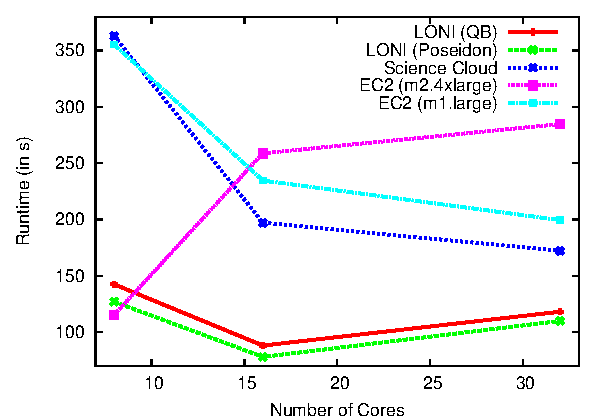
\includegraphics[width=0.45\textwidth]{performance/namd_run.pdf}
    \caption{\textbf{NAMD Runtimes on Different Resource Types: } The
      graph shows that native HPC resource generally outperform Cloud
      resources in particular when running applications across
      multiple nodes. However, the new high memory eight core EC2
      instance type was able to complete a replica run faster than QB
      or Poseidon.}
    \label{fig:performance_namd_run}
\end{figure}

On the HPC resources \tc decreased when using up to 16\,cores. With
more cores a slight increase can be observed. In most EC2 and Nimbus
scenarios the \tc decreased with the number of instances and cores
used. When using the largest EC2 instance~\cite{new-ec2} and increase
of \tc can be observed. These behavior is particularly caused by the
slow interconnects between these instances. Generally those
interconnects are heavily oversubscribed in particular in the EC2
environment causing this massive slowdown. In the following
experiments we will use replica jobs with the size of 8 cores as
basis. In this scenario the cost/performance ratio is particularly in
Clouds optimal.

\subsubsection{\tc for Collective Resource Utilization}

In this scenario we use SAGA BigJob to run replicas across
different types of infrastructures, the LONI
cluster Poseidon, Oliver and the Nimbus Cloud. 
At the beginning of the experiment a particular set of
Pilot-Jobs is started in each environment. Once a Pilot-Job becomes
active, the application assigns replica to this job. 

We measure \tc for different resource configurations using a workload
of 8 replicas each running on 8 cores. The following setups have been used
\begin{itemize}
\item Scenario 1 (A1): Resource I and III -- Clouds and GT2 based Grids. 
\item Scenario 2 (A2): Resource II and III -- Clouds and Condor Grids.
\item Scenario 3 (A3): Resource I, II and III -- Clouds, GT2 and Condor Grids.
\end{itemize} 
For this experiment the LONI clusters: Poseidon and Oliver are used as Grid and Condor resources and
Nimbus as Cloud resource.

\begin{figure}[htbp]
    \centering
        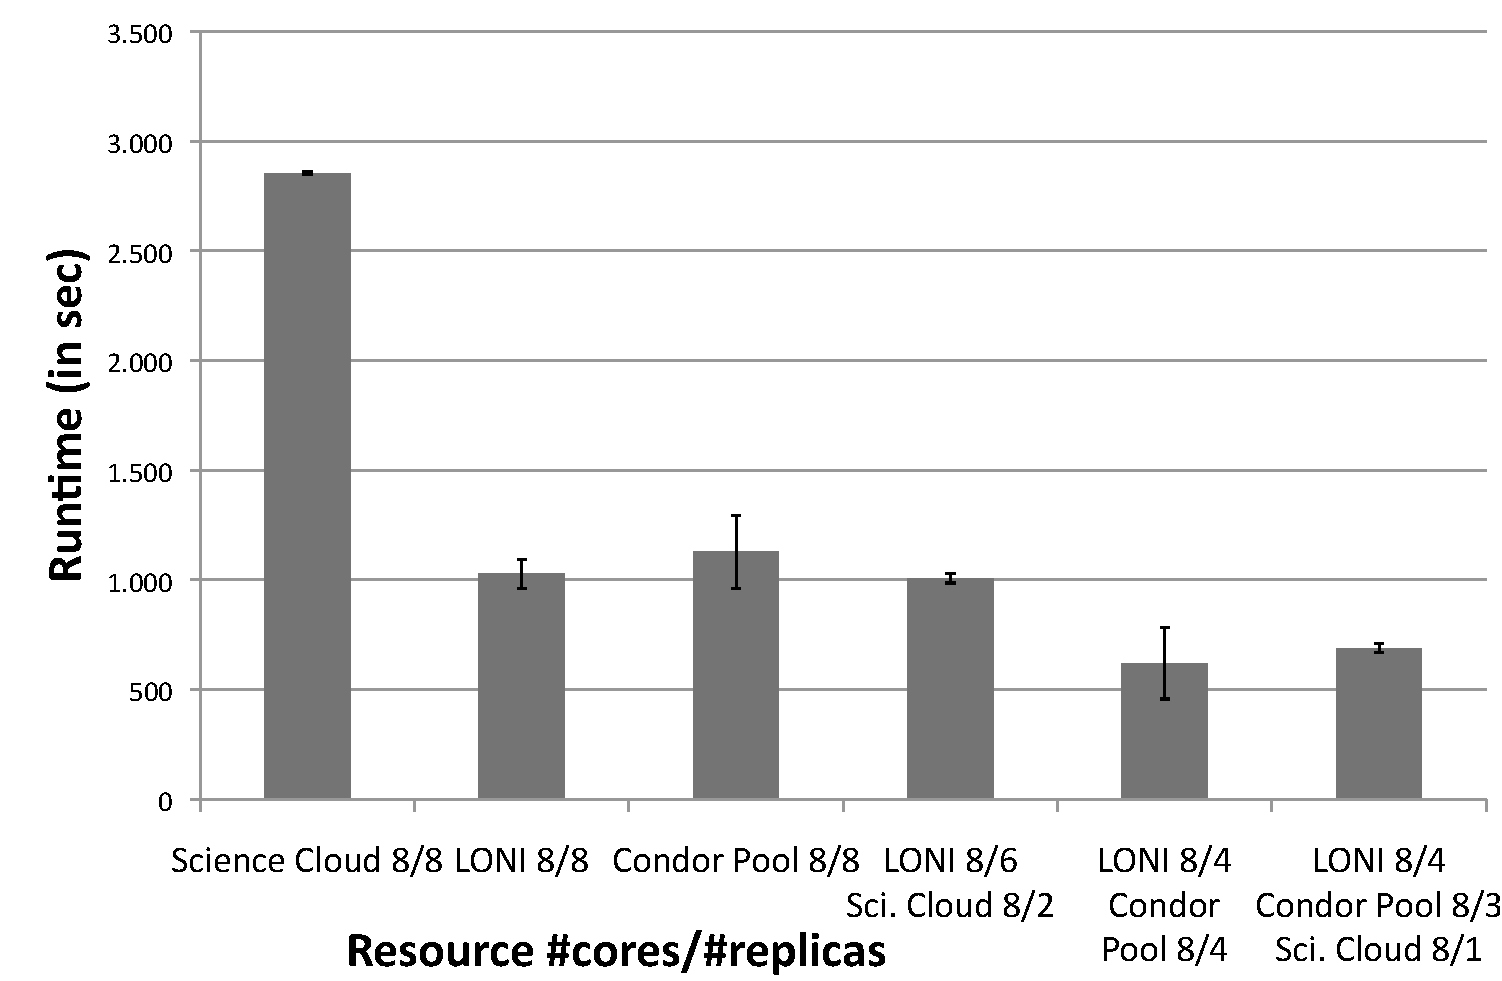
\includegraphics[width=0.47\textwidth]{performance/8replica_scenario_grid_condor_cloud}
        \caption{\textbf{A1 - A3: Collective Usage of Grid, Condor and
            Cloud Resources: } The experiments showed that if the Grid
          and Condor resource Poseidon has only a light load, no
          benefits for using additional Cloud resources
          exist. However, the introduction of an additional Condor
          resp. Grid resource significantly decreases \tc.}
    \label{fig:performance_8replica_grid_cloud_condor}
\end{figure}

Figure~\ref{fig:performance_8replica_grid_cloud_condor} shows the results. 
The performance of the Condor and Grid BigJob is quite similar, which can be expected since the underlying 
physical LONI resources are quite similar. Solely, the slightly higher startup overhead can be observed in the overall Condor
runtime.

In the following the offload of 2 replicas to a Cloud resource has been
investigated. For this purpose, the Nimbus Cloud was used. The offloading of 2 replicas 
to an additional Cloud resource did not result in an 
improved \tc. In such a scenario, \tc is determined by
the slowest resource, i.\,e.\ Nimbus. As described earlier, the
startup time for Nimbus images is in particular for such short runs
significant. Also, NAMD performs significantly worse in the Nimbus
Cloud than on Poseidon or Oliver. Since the startup time on Nimbus
averages to 357\,sec (see Figure~\ref{fig:performance_setup_time}) and
each 8 core replica runs for about 363\,sec (see
Figure~\ref{fig:performance_namd_run}) at least 720\,sec must be
allowed for running a single replica on Nimbus. Thus, it can be
concluded that if resources in the Grids or Condor pool are instantly
available it is not reasonable to start additional Cloud resources.
However, it must be noted that are virtual machines types with a better
performance available, e.\,g.\ in the Amazon Cloud. These VMs 
are usually associated with higher costs (up to 2.40\,\$ per CPU hour) than
the Science Cloud VMs. For a further discussion of cost trade-offs for 
scientific computations in Clouds see Deelman et\,al.~\cite{1413421}. 


\subsection{Scenario B: Investigation of the Distribution of Workload for Maximum Allowed
  Time to Solution} 

Given that Clouds provide the illusion of infinite capacity, or at
least queue wait-times are non-existent, it is likely that often most
sub-jobs will end up on the Cloud infrastructure.  Thus, in Scenario
II, the resource assignment algorithm we use is as follows: We submit
tasks to non-Cloud resources first. Periodically the progress of the
scenario is monitored. If not sufficient jobs have finished
when time equal to $T_{X}$ has elapsed,
%(defined as: \tmax - 2 average \tc on all Clouds)  
than we move the workload to utilize Clouds.  The
underlying basis is that Clouds have an explicit cost associated with
them and if jobs can be completed on the the TG and Condor pool while
preserving the performance constraints, we opt for such a
solution. However, if queue loads prevent the performance requirements
being met, we move the jobs to a Cloud-resource, which we have shown
has less fluctuation in \tc of the workload.

For this experiment we integrated a progress manager that implements
the described algorithm into the replica application.  The user has
the possibility to specify a maximum runtime and a check interval.  At
the beginning of each check interval the progress manager compares the
number of jobs done with the total number of jobs and estimates the
total number of jobs that can be completed within the requested
timeframe. If the total number of jobs is higher than this estimate,
the progress monitor instantiates another BigJob object request
additional Cloud resources for a single replica.  In this scenario,
each time an intermediate target is not met four additional Nimbus VMs
sufficient for running another eight core replica are instantiated.
Table~\ref{tab:app_deadline} summarizes the results.

\begin{table}[ht]
    \centering
	\begin{tabular}{|l|l|l|}
	\hline
    Result & \#\,Occurences &Average \tc \\ \hline
	No VM started &6 &7.8\,min\\ \hline
	1 VMs started &1 &36.4\,min\\ \hline
	2 VMs started &1 &47.3\,min\\ \hline
	3 VMs started &2 &44.2\,min\\ \hline
	\end{tabular}
	\caption{Usage of Cloud Pilot-Jobs to Ensure Deadline \label{tab:app_deadline}}
\end{table}

In the investigated scenario, we configured a maximum runtime of
45\,minutes and a progress check interval of 4 minutes. We repeated
the same experiment 10\,times at different times of the day. In 6 out
of 10\,cases the scenario completed in about 8\,minutes. However, the
fluctuation in particular in the waiting time on typical Grid
resources can be very high. Thus, it was in 4 cases necessary to
start additional VMs to meet the application deadline. 
In two cases 3\,Pilot-Jobs each with 8 cores had to be
started, in one case a single Pilot-Job was sufficient. 
In a single case the deadline was missed
solely due to the fact that not sufficient Cloud resources have been
available, i.\,e.\ we are only able to start 2 instead of 3 Pilot-Jobs. 

\jhanote{Put note to say something about fluctuations on
  Grids/Clusters}. \alnote{done}

\alnote{Old notes: This scenario in particular shows how BigJobs can
  be dynamically created based on runtime decisions.  Based on current
  trends: will we finish or not.  Poseidon BigJob becomes available
  after 100 sec 1 replica finishes after 150 sec After 1/4 check
  whether some resources should be started: - 1 BigJob on Nimbus with
  4 VM - increase VMs linearly if jobs done don't catch - if we caught
  up, we backup}

\section{Other Applications}

\jhanote{Here we should reference the EnKF work, the Replica-Exchange
  work, mention the use with digedag (and Montage in general), support
  for nanoCMOS jobs..}

But mention that this work is different in that, (i) it establishes
the general principles and design, (ii) extends capabilities to work
with Clouds, and (iii) sets the stage for extensible Pilot-Job
functionality, e.g., policy-driven pilot-jobs.

We have discussed how BigJob supports HPC applications; BigJob has
been used to support HTC of HPC applications on the
TeraGrid. Specifically, as shown in Ref.~\cite{enkf-gmac09} the BigJob
has been used to support a very large number of ensembles with highly
variable run-times, as well as heterogenous resource requirements.  In
Ref.~\cite{enkf-gmac09} although efficient scale-out behaviour was
established, all resources utilized were TeraGrid resources, and thus
accessible using a uniform Globus interface. 


Geronimo (an atomic-scale transistor simulator) and RandomSPICE (a
variant of the well-known circuit simulation tool SPICE adapted for
this project). Both use cases are typical parameter sweeps and require
the execution of a very large number of simulations in parallel. To
support these use cases a custom middleware on top of the ScotGrid was
developed. To utilize further distributed resources in the future,
Nano-CMOS~\cite{nanocmos} is currently adopting SAGA. Using the SAGA
framework TeraGrid resources can be used by the electronics engineers
to run their applications.

Need to mention the general purpose nature: both HTC and HTC of HPC,
as well that it is more than just a container of ensemble based
applications.  It provides the framework for deploying and supporting
application-level runtime environments.

\section{Conclusion}

We plan to extend this work in two important directions. The first is
the use of a more sophisticated coordination mechanism -- that
supports asynchronous task coordination (e.g. Comet). In this paper,
we have focussed on replica simulations, but not on replica-exchange
simulations -- which involve coordination between the different tasks
and intelligence in their placements.  It will be very interesting to
note the performance gains that accrue as a result of such
asynchronous coordination on production infrastructure for the
replica-exchange problems. Also, having established the basic
infrastructure to submit tasks to and manage multiple, heterogenous
resources using a simple, single interface, an important second
extension of this work is to use more sophisticated task-placement
decisions or resource utilization decision making.

Programming systems and tools often define the production grid
infrastructure.  The ability to transcend specific programming systems
and utilize existing tools without wholesale refactoring of
applications and application usage-modes is important if not critical
in facilitating the uptake of production grid infrastructure. The
SAGA-based approach outlined here, specifically in the context of
Pilot-Jobs is being used to integrate otherwise disparate PGI such as
the TeraGrid and the OSG, as well as the TeraGrid and EGEE;
application-level interoperability constitutes a different but an
important approach towards the interoperability of PGI.

\begin{acknowledgement}
  \footnotesize{Important funding for SAGA has been provided by the UK
    EPSRC grant number GR/D0766171/1 (via OMII-UK) and HPCOPS NSF-OCI
    0710874. SJ acknowledges the e-Science Institute, Edinburgh for
    supporting the research theme, ``Distributed Programming
    Abstractions'' and theme members for shaping many important
    ideas. This work has also been made possible thanks to the
    internal resources of the Center for Computation \& Technology at
    Louisiana State University and computer resources provided by
    LONI. We thank Yaakoub El Khamra for help with initial experiments
    with the Condor infrastructure. We thank Joohyun Kim (CCT) for
    assistance with the RNA models.}
\end{acknowledgement}



\bibliographystyle{IEEEtran}
\bibliography{literatur,saga}
\end{document}



